\section{Párování}
\subsection{Definice}
Je dán neorientovaný graf $G = (V,E, \eps)$. Podmnožina hran $P \subseteq E$ se nazývá \ii{párování}, jestliže v $P$ 
neexistují 2 různé hrany se společným krajním vrcholem (takže vrchol má stupeň max. 1).

\subsection{Vrchol nasycený a volný v párování}
Mějme párování $P$. Vrchol $v$ grafu nazvěme \ii{nasycený} v $P$, pokud existuje hrana $e \in P$ incidentní s $v$.

V opačném případě říkáme, že vrchol $v$ je \ii{volný} v $P$.
\begin{figure}[H]
    \centering
    \begin{tikzpicture}[
        red_node/.style={circle, draw=red!70, line width=2pt, fill=red!70, minimum size=1mm, inner sep=0pt},
        blue_node/.style={circle, draw=blue!60, line width=2pt, fill=blue!60, minimum size=1mm, inner sep=0pt},
        purple_node/.style={circle, draw=purple, line width=2pt, fill=purple, minimum size=1mm, inner sep=0pt},
        edge_style/.style={draw=black, line width=1pt, line cap=round}
    ]

        \node[red_node] (r_bot_1) at (0, 0) {};
        \node[red_node] (r_bot_2) at (2, 0) {};
        \node[red_node] (r_bot_3) at (4, 0) {};

        \node[red_node] (r_top_1) at (0, 2.5) {};
        \node[red_node] (r_top_2) at (2, 2.5) {};
        \node[red_node] (r_top_3) at (4, 2.5) {};

        \node[blue_node] (b_left)  at (-1, 3.5) {};
        \node[blue_node] (b_right) at (5, -1.0) {};


        \draw[edge_style] (r_bot_1) -- (r_bot_2) -- (r_bot_3);
        \draw[edge_style] (r_top_1) -- (r_top_2) -- (r_top_3);

        \draw[edge_style] (r_bot_1) -- (r_top_1);
        \draw[edge_style] (r_bot_2) -- (r_top_2);
        \draw[edge_style] (r_bot_3) -- (r_top_3);

        \draw[draw=purple, line width=1pt, line cap=round, decoration={snake, amplitude=.4mm}, decorate] (r_bot_1) -- (r_top_1);
        \draw[draw=purple, line width=1pt, line cap=round, decoration={snake, amplitude=.4mm}, decorate] (r_bot_2) -- (r_top_2);
        \draw[draw=purple, line width=1pt, line cap=round, decoration={snake, amplitude=.4mm}, decorate] (r_bot_3) -- (r_top_3);

        \draw[edge_style] (r_bot_1) -- (r_top_2);
        \draw[edge_style] (r_bot_2) -- (r_top_3);

        \draw[edge_style] (b_left) -- (r_top_1);
        \draw[edge_style] (b_right) -- (r_bot_3);

        \matrix [
            % draw=white,
            % fill=white,
            line width=1pt,
            rounded corners=0pt,
            inner sep=2pt,
            row sep=1pt,
            column sep=5pt,
            right=0.5cm of r_top_3,
            anchor=north west
        ] {
            \node[red_node, scale=0.7] {}; & \node[anchor=west] {nasycený}; \\
            \node[blue_node, scale=0.7] {}; & \node[anchor=west] {volný}; \\
            \node[purple_node, scale=0.7] {}; & \node[anchor=west] {párování $P$}; \\
        };
    \end{tikzpicture}
\end{figure}

\subsection{Perfektní párování}
Párování $P$ v grafu $G$ nazveme \ii{perfektní párování}, jestliže každý vrchol grafu je nasycen v $P$. To znamená, že 
$P$ má $\frac{n}{2}$ hran, kde $n$ je počet vrcholů grafu $G$.

\subsection{Maximální párování}
Párování $P$ v grafu $G$ nazveme \ii{maximální párování}, jestliže je nejpočetnější mezi všemi párováními v grafu $G$.

Perfektní párování je jistě maximální. Naopak to neplatí. Existují grafy, které perfektní párování nemají --- stačí 
uvažovat grafy s lichým počtem vrcholů. Ovšem ani grafy se sudým počtem vrcholů nemusí perfektní párování obsahovat.

V každém grafu existuje maximální párování. 

\subsection{Střídavá cesta vůči párování \texorpdfstring{$P$}{P}}
Je dáno párování $P$ v grafu $G$. Cesta $C = e_1, e_2, \dots, e_k$ v grafu $G$ se nazývá \ii{střídavá cesta vůči $P$}, 
jestliže platí následující dvě podmínky:
\begin{enumerate}[1)]
    \item hrany z cesty $C$ střídavě leží a neleží v párování $P$,
    \item jestliže krajní vrchol $v$ cesty $C$ je nasycen v $P$, pak $C$ obsahuje i hranu párování $P$, která vrchol $v$ 
    nasycuje.
\end{enumerate}
\begin{figure}[H]
    \centering
    \begin{tikzpicture}[
        red_node/.style={circle, draw=red!70, line width=2pt, fill=red!70, minimum size=1mm, inner sep=0pt},
        blue_node/.style={circle, draw=blue!60, line width=2pt, fill=blue!60, minimum size=1mm, inner sep=0pt},
        purple_node/.style={circle, draw=purple, line width=2pt, fill=purple, minimum size=1mm, inner sep=0pt},
        green_node/.style={circle, draw=green!70!black, line width=2pt, fill=green!70!black, minimum size=1mm, inner sep=0pt},
        edge_style/.style={draw=black, line width=1pt, line cap=round},
        yellow_edge/.style={draw=green!70!black, line width=1pt, line cap=round}
    ]

        \node[red_node] (r_bot_1) at (0, 0) {};
        \node[red_node] (r_bot_2) at (2, 0) {};
        \node[red_node] (r_bot_3) at (4, 0) {};

        \node[red_node] (r_top_1) at (0, 2.5) {};
        \node[red_node] (r_top_2) at (2, 2.5) {};
        \node[red_node] (r_top_3) at (4, 2.5) {};

        \node[blue_node] (b_left)  at (-1, 3.5) {};
        \node[blue_node] (b_right) at (5, -1.0) {};


        \draw[edge_style] (r_bot_1) -- (r_bot_2) -- (r_bot_3);
        \draw[edge_style] (r_top_1) -- (r_top_2) -- (r_top_3);

        \draw[yellow_edge] (r_bot_1) -- (r_top_1);
        \draw[yellow_edge] (r_bot_2) -- (r_top_2);
        \draw[yellow_edge] (r_bot_3) -- (r_top_3);

        \draw[draw=purple, line width=1pt, line cap=round, decoration={snake, amplitude=.4mm}, decorate] (r_bot_1) -- (r_top_1);
        \draw[draw=purple, line width=1pt, line cap=round, decoration={snake, amplitude=.4mm}, decorate] (r_bot_2) -- (r_top_2);
        \draw[draw=purple, line width=1pt, line cap=round, decoration={snake, amplitude=.4mm}, decorate] (r_bot_3) -- (r_top_3);

        \draw[yellow_edge] (r_bot_1) -- (r_top_2);
        \draw[yellow_edge] (r_bot_2) -- (r_top_3);

        \draw[yellow_edge] (b_left) -- (r_top_1);
        \draw[yellow_edge] (b_right) -- (r_bot_3);

        \matrix [
            % draw=white,
            % fill=white,
            line width=1pt,
            rounded corners=0pt,
            inner sep=2pt,
            row sep=1pt,
            column sep=5pt,
            right=0.5cm of r_top_3,
            anchor=north west
        ] {
            \node[red_node, scale=0.7] {}; & \node[anchor=west] {nasycený}; \\
            \node[blue_node, scale=0.7] {}; & \node[anchor=west] {volný}; \\
            \node[purple_node, scale=0.7] {}; & \node[anchor=west] {párování $P$}; \\
            \node[green_node, scale=0.7] {}; & \node[anchor=west] {střídavá cesta $C$}; \\
        };
    \end{tikzpicture}
\end{figure}

\subsection{Zlepšující cesta vůči párování \texorpdfstring{$P$}{P}}
Střídavá cesta mezi volnými vrcholy se nazývá \ii{zlepšující cesta vůči $P$}.

\subsection{Tvrzení o střídavé cestě}
Jestliže $C$ je střídavá cesta vůči párování $P$, pak množina hran $P^\prime = C \oplus P$ je také párování v $G$.
\ii{Připomeňme, že symetrická diference $A \oplus B$ dvou množin $A, B$ je množina
\begin{equation}
    A \oplus B = (A \cup B) \setminus (A \cap B) = (A \setminus B) \cup (B \setminus A).
\end{equation}
}
\begin{figure}[H]
    \centering
    \begin{minipage}[c]{0.42\textwidth}
        % \begin{figure}[H]
            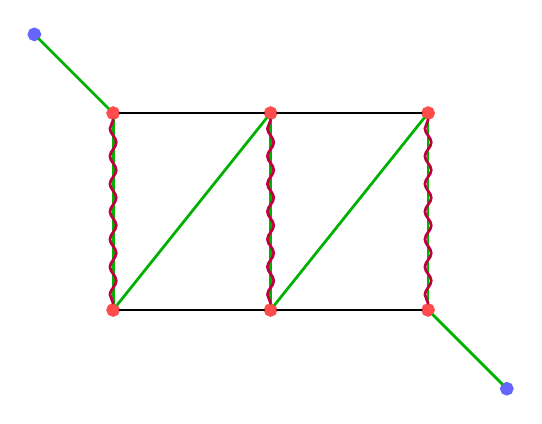
\begin{tikzpicture}[
                red_node/.style={circle, draw=red!70, line width=2pt, fill=red!70, minimum size=1mm, inner sep=0pt},
                blue_node/.style={circle, draw=blue!60, line width=2pt, fill=blue!60, minimum size=1mm, inner sep=0pt},
                purple_node/.style={circle, draw=purple, line width=2pt, fill=purple, minimum size=1mm, inner sep=0pt},
                green_node/.style={circle, draw=green!70!black, line width=2pt, fill=green!70!black, minimum size=1mm, inner sep=0pt},
                edge_style/.style={draw=black, line width=1pt, line cap=round},
                yellow_edge/.style={draw=green!70!black, line width=1pt, line cap=round}
            ]

                \node[red_node] (r_bot_1) at (0, 0) {};
                \node[red_node] (r_bot_2) at (2, 0) {};
                \node[red_node] (r_bot_3) at (4, 0) {};

                \node[red_node] (r_top_1) at (0, 2.5) {};
                \node[red_node] (r_top_2) at (2, 2.5) {};
                \node[red_node] (r_top_3) at (4, 2.5) {};

                \node[blue_node] (b_left)  at (-1, 3.5) {};
                \node[blue_node] (b_right) at (5, -1.0) {};


                \draw[edge_style] (r_bot_1) -- (r_bot_2) -- (r_bot_3);
                \draw[edge_style] (r_top_1) -- (r_top_2) -- (r_top_3);

                \draw[yellow_edge] (r_bot_1) -- (r_top_1);
                \draw[yellow_edge] (r_bot_2) -- (r_top_2);
                \draw[yellow_edge] (r_bot_3) -- (r_top_3);

                \draw[draw=purple, line width=1pt, line cap=round, decoration={snake, amplitude=.4mm}, decorate] (r_bot_1) -- (r_top_1);
                \draw[draw=purple, line width=1pt, line cap=round, decoration={snake, amplitude=.4mm}, decorate] (r_bot_2) -- (r_top_2);
                \draw[draw=purple, line width=1pt, line cap=round, decoration={snake, amplitude=.4mm}, decorate] (r_bot_3) -- (r_top_3);

                \draw[yellow_edge] (r_bot_1) -- (r_top_2);
                \draw[yellow_edge] (r_bot_2) -- (r_top_3);

                \draw[yellow_edge] (b_left) -- (r_top_1);
                \draw[yellow_edge] (b_right) -- (r_bot_3);
            \end{tikzpicture}
        % \end{figure}
    \end{minipage}%
    % \hspace{0.05\textwidth}
    \begin{minipage}[c]{0.55\textwidth}
        % \begin{figure}[H]
            \begin{tikzpicture}[
                red_node/.style={circle, draw=red!70, line width=2pt, fill=red!70, minimum size=1mm, inner sep=0pt},
                blue_node/.style={circle, draw=blue!60, line width=2pt, fill=blue!60, minimum size=1mm, inner sep=0pt},
                purple_node/.style={circle, draw=purple, line width=2pt, fill=purple, minimum size=1mm, inner sep=0pt},
                green_node/.style={circle, draw=green!70!black, line width=2pt, fill=green!70!black, minimum size=1mm, inner sep=0pt},
                cyan_node/.style={circle, draw=cyan!90!black, line width=2pt, fill=green!70!black, minimum size=1mm, inner sep=0pt},
                edge_style/.style={draw=black, line width=1pt, line cap=round},
                cyan_edge/.style={draw=cyan!90!black, line width=1pt, line cap=round}
            ]

                \node[red_node] (r_bot_1) at (0, 0) {};
                \node[red_node] (r_bot_2) at (2, 0) {};
                \node[red_node] (r_bot_3) at (4, 0) {};

                \node[red_node] (r_top_1) at (0, 2.5) {};
                \node[red_node] (r_top_2) at (2, 2.5) {};
                \node[red_node] (r_top_3) at (4, 2.5) {};

                \node[blue_node] (b_left)  at (-1, 3.5) {};
                \node[blue_node] (b_right) at (5, -1.0) {};


                \draw[edge_style] (r_bot_1) -- (r_bot_2) -- (r_bot_3);
                \draw[edge_style] (r_top_1) -- (r_top_2) -- (r_top_3);

                \draw[edge_style] (r_bot_1) -- (r_top_1);
                \draw[edge_style] (r_bot_2) -- (r_top_2);
                \draw[edge_style] (r_bot_3) -- (r_top_3);

                \draw[cyan_edge] (r_bot_1) -- (r_top_2);
                \draw[cyan_edge] (r_bot_2) -- (r_top_3);

                \draw[cyan_edge] (b_left) -- (r_top_1);
                \draw[cyan_edge] (b_right) -- (r_bot_3);

                \matrix [
                    % draw=white,
                    % fill=white,
                    line width=1pt,
                    rounded corners=0pt,
                    inner sep=2pt,
                    row sep=1pt,
                    column sep=5pt,
                    right=0.5cm of r_top_3,
                    anchor=north west
                ] {
                    \node[red_node, scale=0.7] {}; & \node[anchor=west] {nasycený}; \\
                    \node[blue_node, scale=0.7] {}; & \node[anchor=west] {volný}; \\
                    \node[purple_node, scale=0.7] {}; & \node[anchor=west] {párování $P$}; \\
                    \node[green_node, scale=0.7] {}; & \node[anchor=west] {střídavá cesta $C$}; \\
                    \node[cyan_node, scale=0.7] {}; & \node[anchor=west] {párování $P^\prime$}; \\
                };
            \end{tikzpicture}
        % \end{figure}
    \end{minipage}
\end{figure}
A pokud je navíc $C$ zlepšující cesta, tj. cesta mezi volnými vrcholy v $P$, pak $|P^\prime| = |P| + 1$.
